\documentclass[11pt,a4paper]{article}
\usepackage[utf8]{inputenc}
\usepackage[french]{babel}
\usepackage[T1]{fontenc}

\usepackage{amsmath}
\usepackage{amsfonts}
\usepackage{amssymb}

\newcommand{\NomAuteur}{Fabrice BOISSIER}
\newcommand{\TitreMatiere}{Algorithmique 1}
\newcommand{\NomUniv}{EPITA - Bachelor Cyber Sécurité}
\newcommand{\NiveauUniv}{CYBER1}
\newcommand{\NumGroupe}{CYBER1}
\newcommand{\AnneeUniv}{2024-2025}
\newcommand{\DateExam}{juin 2025}
%\newcommand{\TypeExam}{Rattrapage}
\newcommand{\TypeExam}{CORRECTION Rattrap}
\newcommand{\TitreExam}{\TitreMatiere}
\newcommand{\DureeExam}{2h00}
\newcommand{\MyWaterMark}{\AnneeUniv} % Watermark de protection

% Ajout de mes classes & definitions
\usepackage{MetalExam} % Appelle un .sty

% "Tableau" et pas "Table"
\addto\captionsfrench{\def\tablename{Tableau}}

%%%%%%%%%%%%%%%%%%%%%%%
%Header
%%%%%%%%%%%%%%%%%%%%%%%
\lhead{\TypeExam}							%Gauche Haut
\chead{\NomUniv}							%Centre Haut
\rhead{\NumGroupe}							%Droite Haut
\lfoot{\DateExam}							%Gauche Bas
\cfoot{\thepage{} / \pageref*{LastPage}}	%Centre Bas
\rfoot{\texttt{\TitreMatiere}}				%Droite Bas

%%%%%

\usepackage{tabularx}

\newlength{\LabelWidth}%
%\setlength{\LabelWidth}{1.3in}%
\setlength{\LabelWidth}{1cm}%
%\settowidth{\LabelWidth}{Employee E-mail:}%  Specify the widest text here.

% Optional first parameter here specifies the alignment of
% the text within the \makebox.  Default is [l] for left
% alignment. Other options are [r] and [c] for right and center
\newcommand*{\AdjustSize}[2][l]{\makebox[\LabelWidth][#1]{#2}}%


\definecolor{mGreen}{rgb}{0,0.6,0}
\definecolor{mGray}{rgb}{0.5,0.5,0.5}
\definecolor{mPurple}{rgb}{0.58,0,0.82}
\definecolor{backgroundColour}{rgb}{0.95,0.95,0.92}

\lstdefinestyle{CStyle}{
    backgroundcolor=\color{backgroundColour},
    commentstyle=\color{mGreen},
    keywordstyle=\color{magenta},
    numberstyle=\tiny\color{mGray},
    stringstyle=\color{mPurple},
    basicstyle=\footnotesize,
    breakatwhitespace=false,
    breaklines=true,
    captionpos=b,
    keepspaces=true,
    numbers=left,
    numbersep=5pt,
    showspaces=false,
    showstringspaces=false,
    showtabs=false,
    tabsize=2,
    language=C
}


\hyphenation{op-tical net-works SIGKILL}


\begin{document}

\MakeExamTitleDuree     % Pour afficher la duree
%\MakeExamTitle                   % Ne pas afficher la duree

%% \MakeStudentName    %% A reutiliser sur chaque nouvelle page

\bigskip
%\bigskip

Vous devez respecter les consignes suivantes, sous peine de 0 :

\begin{table}[ht!]
  \begin{minipage}{0.45\textwidth}

\begin{enumerate}[label=\Roman*)]
\item Lisez le sujet en entier avec attention
\item Répondez sur le sujet
\item Ne trichez pas
\item Ne détachez pas les agrafes du sujet
\end{enumerate}

  \end{minipage}
  \hfillx
  \begin{minipage}{0.55\textwidth}

\begin{enumerate}[label=\Roman*),start=5]
\item \'Ecrivez lisiblement vos réponses (si nécessaire en majuscules)
%\item Vous devez écrire dans le langage algorithmique classique ou en C (donc pas de Python ou autre)
\item Vous devez écrire les algorithmes et structures en langage C (donc pas de Python ou autre)
\end{enumerate}

  \end{minipage}
\end{table}

%\begin{enumerate}[label=\Roman*)]
%\item Lisez le sujet en entier avec attention
%\item Répondez sur le sujet
%\item Ne détachez pas les agrafes du sujet
%\item \'Ecrivez lisiblement vos réponses (si nécessaire en majuscules)
%%\item Vous devez écrire dans le langage algorithmique classique ou en C (donc pas de Python ou autre)
%\item Vous devez écrire les algorithmes et structures en langage C (donc pas de Python ou autre)
%\item Ne trichez pas
%\end{enumerate}

%\bigskip

%\vfillFirst


\section{Bases d'Algorithmique (10 points)}

\subsection*{Question}

\subsection{(2 points) Exécutez l'algorithme suivant, et notez l'état d'avancement des variables (inscrivez l'état initial dans la ligne prévue à cet effet) : }

\bigskip

\begin{center}
\textit{Vous exécuterez la fonction suivante avec comme paramètres a = 2110 et b = 27972 : }
\end{center}


\begin{table}[h!]
  \centering
  \begin{minipage}{0.59\textwidth}
    \centering

% %*   *)
\begin{lstlisting}[language=C]
int FunctionXYZ(int a, int b)
{
  int num = 0;

  if ((a > 0) && (b < 0))
    return (-1);

  while ((a > 0) && (b > 0))
  {
    if ((num % 2) == 0)
      num += 1;
    else
      num *= 2;
    a = a - 100;
    b = b / 10;
  }
  return (num);
}
\end{lstlisting}

  \end{minipage}
  \hfillx
  \begin{minipage}{0.4\textwidth}
    \centering

    \begin{tabular}{| C{1cm} | C{1cm} | C{1cm} | C{1cm} |}
        \hline
          \cellcolor{black!45} tour  &  \cellcolor{black!15} a  &  \cellcolor{black!15} b  &  \cellcolor{black!15} num  \\
        \hline
        \multirow{2}{*}[0pt]{\textit{\'Etat}}  &      &       &   \\
        \multirow{2}{*}[0pt]{\textit{initial}} & 2110 & 27972 & 0 \\
             &     &     &       \\
        \hline
             &     &     &       \\
          1  & 2010 & 2797 & 1 \\
             &     &     &       \\
        \hline
             &     &     &       \\
          2  & 1910 & 279 & 2 \\
             &     &     &       \\
        \hline
             &     &     &       \\
          3  & 1810 & 27 & 3 \\
             &     &     &       \\
        \hline
             &     &     &       \\
          4  & 1710 & 2 & 6 \\
             &     &     &       \\
        \hline
             &     &     &       \\
          5  & 1610 & 0 & 7 \\
             &     &     &       \\
        \hline
             &     &     &       \\
             &     &     &       \\
             &     &     &       \\
        \hline
             &     &     &       \\
             &     &     &       \\
             &     &     &       \\
        \hline
             &     &     &       \\
             &     &     &       \\
             &     &     &       \\
        \hline
    \end{tabular}
  \end{minipage}

\end{table}


%\vfillLast

\clearpage

%%%%%%%%%%%%%%%%%%%%%%%%%%%%%%%%%%%%%%%%%%%%%%%%%ù

\subsection*{Algorithmes}

\subsection{(2 points) \'Ecrivez une fonction récursive \og \textit{NbChiffres} \fg{} calculant la longueur d'un nombre entier (c'est-à-dire le nombre de chiffres qui le constituent) }

\centerline{\textit{Le nombre \og 0 \fg{} est de longueur 1}}

\medskip

\begin{center}
\GrilleReponseN{10}
\end{center}


%\bigskip


\subsection{(2 points) \'Ecrivez une fonction itérative \og \textit{my\_strlen} \fg{} calculant la taille d'une chaîne de caractères }

\medskip

\begin{center}
\GrilleReponseN{11}
\end{center}


\clearpage

%%%%%%%%%%%%%%%%%%%%%%%%%%%

\subsection{(2 points) \'Ecrivez une fonction \og \textit{Count\_Odd} \fg{} renvoyant la quantité de nombres impairs contenus dans un tableau d'entiers }

\medskip

\begin{center}
%\GrilleReponseN{10}
\GrilleReponseN{8}
\end{center}


%\bigskip


%\subsection{(2 points) Ajoutez la ligne manquante à cet algorithme pour en faire un algorihtme de tri à bulles (on considère que la fonction \og swap \fg{} est disponible) }
\subsection{(2 points) Indiquez et corrigez \underline{la ligne} incorrecte dans ce tri à bulles (on considère que la fonction \og swap \fg{} est disponible) }

\bigskip

%\begin{center}
%\GrilleReponseN{10}
%%\GrilleReponseTextUp{20}{4.3}{\TTBF{\textcolor{blue}{char} *get\_friend(\textcolor{blue}{d\_node} *root, \textcolor{blue}{char} *str)}}
%\end{center}

%%%  if (tab[j] > tab[i])  =>  if (tab[j] > tab[j+1])

% %*   *)
\begin{lstlisting}[language=C,commentstyle=\color{commentgreen}]
void BubbleSort(int tab[], int len)
{

  for (int i = (len - 1); i > 0; i--)
  {

    for (int j = 0; j < i; j++)
    {

%%%%  if (tab[j] > tab[i])         %%%% ERREUR ICI

%     if (tab[j] > tab[j + 1])     % <= CORRECTION

      {

        swap(tab, len, j, (j + 1));

      }

    }

  }

}
\end{lstlisting}


\clearpage

%%%%%%%%%%%%%%%%%%%%%%%%%%%%%%%%%%%%%%%%%%%%%%%%%
%%%%%%%%%%%%%%%%%%%%%%%%%%%%%%%%%%%%%%%%%%%%%%%%%
%%%%%%%%%%%%%%%%%%%%%%%%%%%%%%%%%%%%%%%%%%%%%%%%%

\section{Listes/Piles/Files (7 points)}

\subsection*{Questions}

%\subsection{(1 point) \'Ecrivez l'état d'une file après avoir effectué ces opérations (la file est considérée comme initialement vide) : }
\subsection{(1 point) \'Ecrivez l'état d'une file après avoir effectué ces opérations (la file est considérée comme initialement vide), puis, indiquez quel élément sortira de la file lors du prochain \og dequeue \fg{}, ainsi que celui qui sortira en dernier : }

\bigskip

\begin{center}

\begin{large}
%enfiler 2, enfiler 4, défiler, enfiler 3, enfiler 1, défiler, défiler, enfiler 7, enfiler 5, défiler, enfiler 6
enfiler 3, enfiler 1, enfiler 4, défiler, enfiler 2, défiler, défiler, enfiler 6, enfiler 7, défiler, enfiler 5
\end{large}

\bigskip

\begin{tabular}{ | C{1cm} | C{1cm} | C{1cm} | C{1cm} | C{1cm} | C{1cm} | }
  \hline
  \cellcolor{black!0}   & \cellcolor{black!0}   & \cellcolor{black!0}   & \cellcolor{black!0}   & \cellcolor{black!0}   & \cellcolor{black!0}   \\
  \cellcolor{black!0} 6  & \cellcolor{black!0} 7  & \cellcolor{black!0} 5  & \cellcolor{black!0}   & \cellcolor{black!0}   & \cellcolor{black!0}   \\
  \cellcolor{black!0}   & \cellcolor{black!0}   & \cellcolor{black!0}   & \cellcolor{black!0}   & \cellcolor{black!0}   & \cellcolor{black!0}   \\
  \hline
\end{tabular}

\smallskip

\begin{tabular}{   C{1cm}   C{1cm}   C{1cm}   C{1cm}   C{1cm}   C{1cm}   }
  \tikzarrowup{middarkgreen}{middarkgreen}{\phantom{cf}} &  &  &  &  &  \\
  Head &  &  &  &  &  \\
\end{tabular}


%\begin{center}
\begin{table}[ht!]
%  \centering
  \begin{minipage}{0.50\textwidth}

Prochain élément qui sortira : \hspace*{1cm} 6

  \end{minipage}
  \hfillx
  \begin{minipage}{0.50\textwidth}

Dernier élément qui sortira : \hspace*{1cm} 5

  \end{minipage}
\end{table}
\end{center}


\bigskip


\vfillFirst

%%%%%%%%%%%%%%%%%%%%%%%%%%%%%%%%%%%%%%%%%%%%%%%%%%%%%%%%%%%%%%%%%%%%%%%
%%%%%%%%%%%%%%%%%%%%%%%%%%%%%%%%%%%%%%%%%%%%%%%%%%%%%%%%%%%%%%%%%%%%%%%

%\subsection{(1 point) \'Ecrivez l'état d'une pile après avoir effectué ces opérations (la pile est considérée comme initialement vide) : }
\subsection{(1 point) \'Ecrivez l'état d'une pile après avoir effectué ces opérations (la pile est considérée comme initialement vide), puis, indiquez quel élément sortira de la pile lors du prochain \og pop \fg{}, ainsi que celui qui sortira en dernier : }

\bigskip

\begin{center}

\begin{large}
%empiler 2, empiler 4, dépiler, empiler 3, empiler 1, dépiler, dépiler, empiler 7, empiler 5, dépiler, empiler 6
empiler 5, empiler 3, empiler 2, dépiler, dépiler, empiler 4, dépiler, dépiler, empiler 1, \linebreak empiler 6, dépiler, empiler 7
\end{large}

\bigskip

\begin{tabular}{ | C{1cm} | C{1cm} | C{1cm} | C{1cm} | C{1cm} | C{1cm} | }
  \hline
  \cellcolor{black!0}   & \cellcolor{black!0}   & \cellcolor{black!0}   & \cellcolor{black!0}   & \cellcolor{black!0}   & \cellcolor{black!0}   \\
  \cellcolor{black!0} 1  & \cellcolor{black!0} 7  & \cellcolor{black!0}   & \cellcolor{black!0}   & \cellcolor{black!0}   & \cellcolor{black!0}   \\
  \cellcolor{black!0}   & \cellcolor{black!0}   & \cellcolor{black!0}   & \cellcolor{black!0}   & \cellcolor{black!0}   & \cellcolor{black!0}   \\
  \hline
\end{tabular}

\smallskip

\begin{tabular}{   C{1cm}   C{1cm}   C{1cm}   C{1cm}   C{1cm}   C{1cm}   }
  &  & \tikzarrowup{middarkgreen}{middarkgreen}{\phantom{cf}} &  &  &  \\
  &  & Head &  &  &  \\
\end{tabular}


%\begin{center}
\begin{table}[ht!]
%  \centering
  \begin{minipage}{0.50\textwidth}

Prochain élément qui sortira : \hspace*{1cm} 7

  \end{minipage}
  \hfillx
  \begin{minipage}{0.50\textwidth}

Dernier élément qui sortira : \hspace*{1cm} 1

  \end{minipage}
\end{table}
\end{center}


\bigskip


\vfillLast

%%%%%%%%%%%%%%%%%%%%%%%%%%%%%%%%%%%%%%%%%%%%%%%%%%%%%%%%%%%%%%%%%%%%%%%
%%%%%%%%%%%%%%%%%%%%%%%%%%%%%%%%%%%%%%%%%%%%%%%%%%%%%%%%%%%%%%%%%%%%%%%

\subsection{(0,5 point) Déduisez maintenant la caractéristique de chacun des conteneurs : }

%\bigskip

\begin{center}
\begin{table}[ht!]
%  \centering
  \begin{minipage}{0.50\textwidth}
  \centering

\begin{tabular}{|L{5cm}|L{2cm}|}
\hline
\multirow{3}{*}[0pt]{\begin{minipage}{4.85cm} Ce conteneur maintient en sortie l'ordre dans lequel les éléments sont insérés \end{minipage}}
 & \\
 & FILE \\
 & \\
\hline
\end{tabular}

  \end{minipage}
  \hfillx
  \begin{minipage}{0.50\textwidth}
  \centering

\begin{tabular}{|L{5cm}|L{2cm}|}
\hline
\multirow{3}{*}[0pt]{\begin{minipage}{4.85cm} Ce conteneur modifie en sortie l'ordre dans lequel les éléments sont insérés \end{minipage}}
 & \\
 & PILE \\
 & \\
\hline
\end{tabular}

  \end{minipage}
\end{table}
\end{center}


\clearpage
%%%%%%%%%%%%%%%%%%%%%%%%%%%%%%%%%%%%%%%%%%%%%%%%%%%%%%%%%%%%%%%%%%%%%%%

\subsection{(1,5 point) En admettant que l'on dispose d'une pile vide et que les éléments \og 1 2 3 4 5 6 \fg{} arrivent en entrée dans cet ordre exclusivement, décrivez les scénarios permettant d'obtenir les sorties suivantes. Si c'est impossible, indiquez simplement \og impossible \fg{}  : }

%\medskip
\smallskip

\begin{center}
\noindent \textit{exemple : pour \og A B C \fg{} en entrée, on peut obtenir \og B C A \fg{} en sortie en faisant : \linebreak
\og push A \fg, \og push B \fg, \og pop \fg, \og push C \fg, \og pop \fg, \og pop \fg }

\noindent \textit{On a bien inséré A, puis B, puis C, mais l'ordre de sortie est différent suivant les \og pop \fg}
\end{center}


\begin{center}

\begin{large}
%2, 1, 3, 6, 5, 4
3, 4, 5, 2, 6, 1
\end{large}

\begin{center}
%\GrilleReponseN{6}
 push 1, push 2, push 3, pop, push 4, pop, push 5, pop, pop, push 6, pop, pop
\end{center}

\vspace*{3cm}

\begin{large}
%4, 3, 5, 2, 1, 6
1, 3, 5, 2, 4, 6
\end{large}

\begin{center}
%\GrilleReponseN{6}
 impossible
\end{center}

\vspace*{3cm}

\begin{large}
%2, 4, 3, 5, 6, 1
2, 5, 4, 6, 3, 1
\end{large}

\begin{center}
%\GrilleReponseN{6}
 push 1, push 2, pop, push 3, push 4, push 5, pop, pop, push 6, pop, pop, pop
\end{center}

\end{center}



\clearpage

%%%%%%%%%%%%%%%%%%%%%%%%%%%%%%%%%%%%%%%%%%%%%%%%%%%%%%%%%%%%%%%%%%%%%%%%%%%%%%%%%%%%
%%%%%%%%%%%%%%%%%%%%%%%%%%%%%%%%%%%%%%%%%%%%%%%%%%%%%%%%%%%%%%%%%%%%%%%%%%%%%%%%%%%%
\subsection*{Algorithmes}

\begin{center}
\begin{table}[ht!]
%  \centering
  \begin{minipage}{0.48\textwidth}

\subsection{(0,5 point) \'Ecrivez une structure de données \og \textit{my\_stack} \fg{} pouvant servir de pile (à base de pointeurs ou de tableaux) }

\medskip

\begin{center}
%\GrilleReponseN{7}
\GrilleReponseXY{8}{8}
\end{center}

  \end{minipage}
  \hfillx
  \begin{minipage}{0.48\textwidth}

\subsection{(0,5 point) \'Ecrivez une structure de données \og \textit{my\_queue} \fg{} pouvant servir de file (à base de pointeurs ou de tableaux) }

\medskip

\begin{center}
%\GrilleReponseN{7}
\GrilleReponseXY{8}{8}
\end{center}

  \end{minipage}
\end{table}
\end{center}


\vspace*{-0.5cm}


%%%%%%%%%%%%%%%%%%%%%%%%%%%%%%%%%%%%%%%%%%%%%%%%%%%%%%%%

\begin{center}
\begin{table}[ht!]
%  \centering
  \begin{minipage}{0.48\textwidth}

\subsection{(1 point) \'Ecrivez une fonction \og \textit{push} \fg{} pouvant servir à empiler un élément dans votre précédente structure \og \textit{my\_stack} \fg{} }

\medskip

\begin{center}
%\GrilleReponseN{7}
\GrilleReponseXY{8}{10}
\end{center}

  \end{minipage}
  \hfillx
  \begin{minipage}{0.48\textwidth}

\subsection{(1 point) \'Ecrivez une fonction \og \textit{pop} \fg{} pouvant servir à dépiler un élément dans votre précédente structure \og \textit{my\_stack} \fg{} }

\medskip

\begin{center}
%\GrilleReponseN{7}
\GrilleReponseXY{8}{10}
\end{center}

  \end{minipage}
\end{table}
\end{center}


\clearpage

%%%%%%%%%%%%%%%%%%%

\section{Problème : Ordonnancement (3 points)}

\noindent L'ordonnanceur d'un système d'exploitation est un composant distribuant du temps d'exécution à chaque tâche selon divers critères dont la priorité.
Dans le problème traité ici, seuls deux critères nous intéressent : la \textit{priorité} du processus, et la \textit{durée d'exécution} totale déjà réalisée.

\medskip

\noindent Dans un ordonnanceur, les nouveaux processus sont ajoutés au fur et à mesure dans la file d'attente, mais, on n'attribue du temps qu'à celui qui est en tête de la file.
L'insertion dans la file d'attente n'est pas une insertion classique en queue, mais plutôt n'importe où dans la file selon des critères.

\medskip

\noindent Ici, le critère le plus important sera la \textit{priorité} : plus la valeur de priorité est basse, moins le processus devra attendre pour être exécuté (il sera donc très prioritaire).
Exemple : un processus avec une priorité de 2 attendra moins qu'un processus avec une priorité de 5.
La valeur de priorité est un entier positif (0 étant la plus petite valeur, et donc, la priorité maximale).

\medskip

\noindent Le deuxième critère est la \textit{durée d'exécution} totale déjà réalisée : plus un processus va prendre de temps d'exécution, moins il sera prioritaire (les tâches récentes passeront avant les plus anciennes).
Exemple : un processus avec une priorité de 4 ayant été exécuté seulement 7 minutes attendra moins qu'un processus avec une priorité de 4 ayant été exécuté 21 minutes, mais, il attendra toujours plus qu'un processus de priorité 1 ayant été exécuté 42 minutes.

\medskip

\noindent Enfin, si une tâche déjà présente dans la file d'attente a les mêmes caractéristiques, la nouvelle tâche passera après (en d'autres termes : si deux processus ont les mêmes priorités et temps d'exécution, alors le premier arrivé est le premier servi).

\bigskip

\noindent Pour résoudre ce problème, vous avez accès à cette structure \TTBF{struct task\_struct} décrivant une tâche/un processus :
% %*   *)
\begin{lstlisting}[language=C,commentstyle=\color{commentgreen}]
struct task_struct
{
  void  *stack;
  int   PID;    // Identifiant du processus
  int   prio;   // Priorite
  int   usage;  // Temps total d'execution
}; \end{lstlisting}



\noindent Dans ce problème, il faut donc trouver l'emplacement idéal dans un \TTBF{struct task\_struct**}, c'est-à-dire un tableau de \TTBF{struct task\_struct*}.
La taille du tableau est maintenue dans un paramètre.
L'exemple suivant illustre une tâche \textit{T\_H} de priorité 3, et de durée totale 1 minute, insérée avant la tâche \textit{T\_C} de priorité 3 et de durée totale 10 minutes, mais après la tâche \textit{T\_A} de priorité 2 et de durée totale 15 minutes.
La file d'attente est toujours triée dans le bon ordre, et elle doit donc le rester grâce à vos fonctions.


\begin{center}
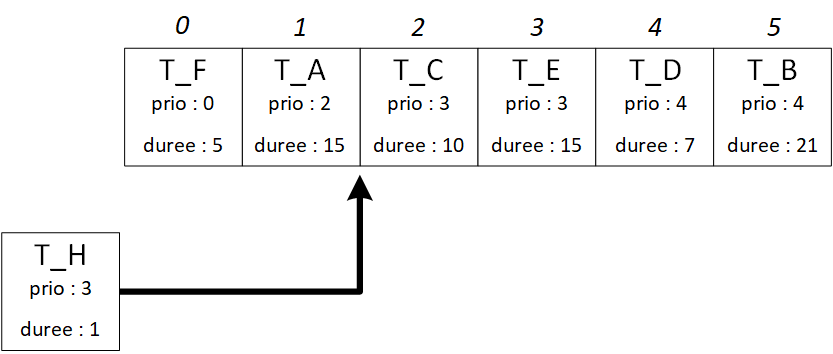
\includegraphics[scale=1.25]{./img/example_scheduling.png}
\end{center}


\medskip


%\noindent Vous allez devoir insérer successivement des processus dans une file d'attente en vous servant de la fonction \TTBF{InsertList(list *L, int elt, int pos)}.
%Cette fonction a déjà été implémentée, vous n'avez qu'à l'utiliser dans un algorithme dont le but est de choisir la position à donner en paramètre de \TTBF{InsertList}.
%Les paramètres sont les suivants :
%\begin{itemize}
%\item \textit{list *L} : le conteneur où insérer le nouvel élément (ici la file d'attente)
%\item \textit{int elt} : l'élément à insérer (ici l'identifiant du processus)
%\item \textit{int pos} : la position dans le conteneur (\textit{0} étant la tête/le prochain élément défilé)
%\end{itemize}
%
\noindent Vous avez également le droit d'utiliser la fonction \TTBF{InsertList} prenant ces paramètres : \linebreak

\noindent \TTBF{InsertList(struct task\_struct **L, struct task\_struct *elt, int pos)}
\begin{itemize}
\item \textit{struct task\_struct **L} : le conteneur où insérer le nouvel élément (ici la file d'attente)
\item \textit{struct task\_struct *elt} : l'élément à insérer (ici la structure concernant le processus)
\item \textit{int pos} : la position dans le conteneur (\textit{0} étant la tête/le prochain processus à être exécuté)
\end{itemize}


%%%%%%%%%%%%%%%%%%%%%%%%%

\subsection{(2 points) \'Ecrivez d'abord une fonction parcourant la file d'attente pour trouver la position du nouveau processus selon les critères précédents : }

\medskip

\begin{center}
%\GrilleReponseN{13}
%\GrilleReponseTextUp{20}{4.3}{\TTBF{\textcolor{blue}{int} calculate\_position(\textcolor{blue}{struct task\_struct} **sched\_list, \textcolor{blue}{int} sched\_list\_len, \textcolor{blue}{struct task\_struct} *new\_task)}}
%
\begin{tikzpicture}
\draw[step=0.5cm, lightgray, very thin] (0, 0) grid (16, 20);
\node[draw=none, align=left, label={right:\TTBF{\textcolor{blue}{int} CalculatePosition(\textcolor{blue}{struct task\_struct} **sched\_list,}}] at (0, 20.0 - 0.25) {};
\node[draw=none, align=left, label={right:\TTBF{\hspace*{4.85cm} \textcolor{blue}{int} sched\_list\_len,}}] at (0, 19.5 - 0.25) {};
\node[draw=none, align=left, label={right:\TTBF{\hspace*{4.85cm} \textcolor{blue}{struct task\_struct} *new\_task)}}] at (0, 19.0 - 0.25) {};
\end{tikzpicture}
\end{center}

%%%%%%%%%%%%%%%%%%%%%%%%%

\subsection{(1 point) \'Ecrivez ensuite une fonction insérant le processus à sa place et renvoyant la nouvelle taille de la liste : }

\medskip

\begin{center}
%\GrilleReponseN{13}
\GrilleReponseTextUp{24}{0}{\TTBF{\textcolor{blue}{int} InsertProcess(\textcolor{blue}{struct task\_struct} **sched\_list,} \\
\hspace*{4cm} \TTBF{\textcolor{blue}{int} sched\_list\_len,} \\
\hspace*{4cm} \TTBF{\textcolor{blue}{struct task\_struct} *new\_task)}}
\end{center}


%%%%%%%%%%%%%%%%%%%%%%%%%%%%%%%%%%%%%%%%%%%%%%%%%%%%%%%%
%%%%%%%%%%%%%%%%%%%%%%%%%%%%%%%%%%%%%%%%%%%%%%%%%%%%%%%%
%%%%%%%%%%%%%%%%%%%%%%%%%%%%%%%%%%%%%%%%%%%%%%%%%%%%%%%%

\clearpage

%\thispagestyle{empty}

\vfillFirst

\begin{center}

\begin{LARGE}
\textbf{SUJET RATTRAPAGE}

\bigskip

\textbf{\MakeUppercase{\TitreMatiere}}
\end{LARGE}

\end{center}

\vfillLast

\end{document}
